\renewcommand{\this}{BayesianNetworks}

\chapter{Bayesian Networks}
This chapter is partially based on 
\textit{A Tutorial on Learning With Bayesian Networks} and Christopher
M. Bishops classic \textit{Pattern Recognition and Machine Learning}.
\\\\
In this chapter, we will go over the basics of 
Bayesian networks. In essence, Bayesian networks
are a compact representation over a set of
random variables. They are a subset of the so called
Probabilistic Graphical Models (PGM) which are more
commonly referred to as graphical models. Graphical
models express conditional independence between 
variables using graphs, hence their name.
Bayesian networks have become somewhat popular and
used in quite a few applications. Many libraries
provide easy development using Bayesian networks.
\\\\
This section is structured as follows. First we delve
deeper into \textit{directed acyclic graphs} (DAGs), which
is used to encode conditional independence in Bayesian
networks. We look into the definition of Bayesian,
which turn out to be quite simple yet elegant. A
big downside to Bayesian networks, however, is the
computational complexity. Thirdly, we have a look 
at exact inference in Bayesian networks. Then we
look at approximate inference.

\section{Conditional independence as a DAG}
Graphical models are based on graphs to encode conditional independence 
in probability distributions. In the case of Bayesian networks conditional
independence is encoded as a \textit{directed acyclic graph}, or more 
commonly referred to as DAGs. DAGs are defined as follows:

\begin{defn}[Directed Acyclic Graph]
A graph $G = (V, E)$ is called acyclic when the edges $E$ are directed
and the graph contains no directed cycles. A directed cycle is a 
sequence of connected edges such that at least one vertex is visited 
twice.
\begin{equation}
\lnot \exists x_1, x_2 \dots x_n \in V: (x_i, x_{i+1}) \in E \text{ and }
	x_1 = x_n
\end{equation}
\end{defn}

\noindent
As an example figure \ref{fig:example_DAG} shows two graphs 
over the vertex set $V=\{A, B, C, D\}$. The left graph is a DAG
as there is no vertex from which there is a sequence of directed
edges which result in the same vertex. The right graph does 
contain a directed cycle. For example the path defined by $ACDA$.

\begin{figure}[h!]
\centering

\begin{minipage}[c]{0.3\textwidth}
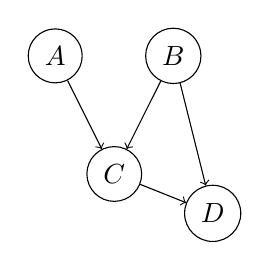
\begin{tikzpicture}
	\draw (0,0) node[shape=circle, draw=black](a){$A$};
	\draw (1.5,0) node[shape=circle, draw=black](b){$B$};
	\draw (0.75,-1.5) node[shape=circle, draw=black](c){$C$};
	\draw (2,-2) node[shape=circle, draw=black](d){$D$};
	
	\draw [->](a) -- (c);
	\draw [->](b) -- (c);
	\draw [->](b) -- (d);
	\draw [->](c) -- (d);
\end{tikzpicture}
\end{minipage}
\begin{minipage}[c]{0.3\textwidth}
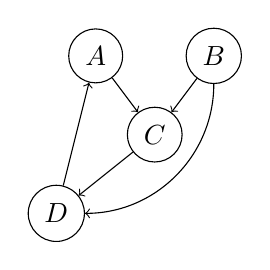
\begin{tikzpicture}

	\draw (0,0) node[shape=circle, draw=black](a){$A$};
	\draw (1.5,0) node[shape=circle, draw=black](b){$B$};
	\draw (0.75,-1.0) node[shape=circle, draw=black](c){$C$};
	\draw (-0.5,-2) node[shape=circle, draw=black](d){$D$};
	
	\draw [->](a) -- (c);
	\draw [->](b) -- (c);
	\draw [->](b.south) to [out=270, in= 0] (d.east);
	\draw [->](c) -- (d);
	\draw [->](d) -- (a);
\end{tikzpicture}
\end{minipage}
\caption{Example of a DAG (left) and a graph with a directed
cycle (right).}
\label{fig:example_DAG}
\end{figure}

\noindent
Two important concepts in DAGs is the concept of parents, children 
and descendants.
\begin{defn}[Parents]
Given a vertex $v \in V$ in a DAG $G=(V, E)$ the parents of 
$v$ are all the vertices for which an outgoing edge ends in $v$:
\begin{equation}
Pa(v) = \{ u \in V \mid (u, v) \in E\}
\end{equation}
\end{defn}

\begin{defn}[Children]
Given a vertex $v \in V$ in a DAG $G=(V, E)$ the children of 
$v$ are all the vertices $u$ in which an outgoing edge of $v$
ends.
\begin{equation}
C(v) = \{ u \in V \mid (v, u) \in E\}
\end{equation}
\end{defn}

\begin{defn}[Descendants]
Given a vertex $v \in V$ in a DAG $G=(V, E)$ the descendants of 
$v$ are all its children and recursively the descendants of all its 
children.
\begin{equation}
Des(v) = \bigcup_{u \in C(v)} Des(u) \cup C(v)
\end{equation}
\end{defn}

\noindent
Figure \ref{fig:exmpl_child_parent_des} shows the parents, children
and descendants of node $v$ in a DAG.

\begin{figure}[h!]
\begin{minipage}[c]{0.32\textwidth}
\scalebox{0.9}{\begin{tikzpicture}

	\node[cloud, 
		  draw, 
		  cloud puffs = 15, 
		  minimum width = 4cm, 
		  aspect = 1.4](cloud) at (1.15,1.2){parents};
	\draw (0,0) node[draw = black,
			   		 shape = circle](p1){$p_1$};
	\draw (1.15,0) node[](1){$\dots$};
	\draw (2.3,0) node[draw = black,
			   		 shape = circle](p2){$p_n$};
	
	\draw (1.15,-1) node[draw = black,
			   		 	shape = circle](v){$v$};
	\draw (0,-2) node[draw = black,
			   		 shape = circle](c1){$c_1$};
	\draw (1.15,-2) node[](1){$\dots$};
	\draw (2.3,-2) node[draw = black,
			   		 shape = circle](c2){$c_n$};
	\node[cloud, 
	  draw, 
	  cloud puffs = 15, 
	  minimum width = 4cm, 
	  aspect = 1.4](cloudC) at (1.15,-3.4){children};
			   		 
	\draw[->] (-0.4, 0.8) -- (p1);
	\draw[->] (0.4, 0.64) -- (p1);
	
	\draw[->] (1.9, 0.64) -- (p2);
	\draw[->] (2.7, 0.8) -- (p2);
	
	\draw[->] (p1) -- (v);
	\draw[->] (p2) -- (v);
	
	\draw[->] (v) -- (c1);
	\draw[->] (v) -- (c2);
	
	\draw[->] (c1) -- (-0.37, -2.8);
	\draw[->] (c1) -- (0.37, -2.6);
	
	\draw[->] (c2) -- (1.93, -2.6);
	\draw[->] (c2) -- (2.67, -2.8);
	
	\draw [draw=red, 
		   rounded corners, 
		   very thick] (-0.5, -0.5) rectangle(2.8, 0.5);
			   		 
\end{tikzpicture}}
\end{minipage}
\begin{minipage}[c]{0.32\textwidth}
\scalebox{0.9}{\begin{tikzpicture}

	\node[cloud, 
		  draw, 
		  cloud puffs = 15, 
		  minimum width = 4cm, 
		  aspect = 1.4](cloud) at (1.15,1.2){parents};
	\draw (0,0) node[draw = black,
			   		 shape = circle](p1){$p_1$};
	\draw (1.15,0) node[](1){$\dots$};
	\draw (2.3,0) node[draw = black,
			   		 shape = circle](p2){$p_n$};
	
	\draw (1.15,-1) node[draw = black,
			   		 	shape = circle](v){$v$};
	\draw (0,-2) node[draw = black,
			   		 shape = circle](c1){$c_1$};
	\draw (1.15,-2) node[](1){$\dots$};
	\draw (2.3,-2) node[draw = black,
			   		 shape = circle](c2){$c_n$};
	\node[cloud, 
	  draw, 
	  cloud puffs = 15, 
	  minimum width = 4cm, 
	  aspect = 1.4](cloudC) at (1.15,-3.4){children};
			   		 
	\draw[->] (-0.4, 0.8) -- (p1);
	\draw[->] (0.4, 0.64) -- (p1);
	
	\draw[->] (1.9, 0.64) -- (p2);
	\draw[->] (2.7, 0.8) -- (p2);
	
	\draw[->] (p1) -- (v);
	\draw[->] (p2) -- (v);
	
	\draw[->] (v) -- (c1);
	\draw[->] (v) -- (c2);
	
	\draw[->] (c1) -- (-0.37, -2.8);
	\draw[->] (c1) -- (0.37, -2.6);
	
	\draw[->] (c2) -- (1.93, -2.6);
	\draw[->] (c2) -- (2.67, -2.8);
			   		 
	\draw [draw=red, 
		   rounded corners, 
		   very thick] (-0.5, -2.5) rectangle (2.8, -1.5);
\end{tikzpicture}}
\end{minipage}
\begin{minipage}[c]{0.32\textwidth}
\scalebox{0.9}{
\begin{tikzpicture}

	\node[cloud, 
		  draw, 
		  cloud puffs = 15, 
		  minimum width = 4cm, 
		  aspect = 1.4](cloud) at (1.15,1.2){parents};
	\draw (0,0) node[draw = black,
			   		 shape = circle](p1){$p_1$};
	\draw (1.15,0) node[](1){$\dots$};
	\draw (2.3,0) node[draw = black,
			   		 shape = circle](p2){$p_n$};
	
	\draw (1.15,-1) node[draw = black,
			   		 	shape = circle](v){$v$};
	\draw (0,-2) node[draw = black,
			   		 shape = circle](c1){$c_1$};
	\draw (1.15,-2) node[](1){$\dots$};
	\draw (2.3,-2) node[draw = black,
			   		 shape = circle](c2){$c_n$};
	\node[cloud, 
	  draw, 
	  cloud puffs = 15, 
	  minimum width = 4cm, 
	  aspect = 1.4](cloudC) at (1.15,-3.4){children};
			   		 
	\draw[->] (-0.4, 0.8) -- (p1);
	\draw[->] (0.4, 0.64) -- (p1);
	
	\draw[->] (1.9, 0.64) -- (p2);
	\draw[->] (2.7, 0.8) -- (p2);
	
	\draw[->] (p1) -- (v);
	\draw[->] (p2) -- (v);
	
	\draw[->] (v) -- (c1);
	\draw[->] (v) -- (c2);
	
	\draw[->] (c1) -- (-0.37, -2.8);
	\draw[->] (c1) -- (0.37, -2.6);
	
	\draw[->] (c2) -- (1.93, -2.6);
	\draw[->] (c2) -- (2.67, -2.8);
			   		 
	\draw [draw=red, 
		   rounded corners, 
		   very thick] (-1, -1.5) rectangle (3.3, -4.5);
\end{tikzpicture}}
\end{minipage}
\caption{Visualization of parents $Pa(v)$, children $C(v)$ and
descendants $Des(v)$ of a node $v$ in a DAG.}
\label{fig:exmpl_child_parent_des}
\end{figure}

\section{Bayesian networks with DAGs}
What do these DAGs have to do with Bayesian networks? As mentioned
earlier in the context of Bayesian networks they define conditional
independence between variables. Let us first define Bayesian networks:

\begin{defn}[Bayesian networks]
A Bayesian network over variables $\textbf{X}=\{X_1,\dots X_k\}$
is a graph-probability pair $(G, \Theta)$. The graph $G$ is a DAG
which encodes conditional independence. The vertices $V$ in $G$ are
in a one-to-one correspondence with the variables $\textbf{X}$. We
do not make a distinction between the random variable $X_i \in 
\textbf{X}$ and the graph node $X_i \in V$. In this definition 
$\Theta$ is a collection of local conditional probabilities for 
each variable $X_i \in \textbf{X}$. The set $\Theta$ is defined as:
\begin{equation}
\Theta = \{P(X_i | Pa(X_i)) | X_i \in \textbf{X}\}
\end{equation}
Together, $G$ and $\Theta$ define a joint probability distribution
over the variables $\textbf{X}$:
\begin{equation}
p(\textbf{X} = x) = \prod_{i=1}^{k} p(X_i = x_i | Pa(X_i) = x)
\end{equation}
\end{defn}

\begin{exmp}
This example was taken from Christopher M. Bishop's classic book
\textit{pattern recognition and machine learning}. Let's assume
we are tasked with fitting a polynomial regression to a data set 
$\textbf{x} = \{x_1, \dots, x_n\}$ where $x_i \in \Real^m$ and 
observations $\textbf{y}=\{y_1, \dots, y_n\}$ and wish to predict 
a given new point $x_{n+1}$.
In the case of Bayesian learning, the model parameters $\textbf{W}$
and observations $\textbf{Y}$ will be considered as random variables.
Hence, we also assume a prior over $\textbf{W}$. This prior has one
hyper parameter $\alpha$ and is written as $p(\textbf{W} \mid \alpha)$.
Additionally, the noise parameter $\sigma^2$ and $\alpha$ are
considered known and fixed. The joint distribution over $\textbf{W}$ 
and $\textbf{Y}$ is then:

\begin{equation}
\begin{split}
p(\textbf{W}, \textbf{Y} \mid \textbf{x}, \alpha, \sigma^2) 
	&= p(\textbf{W} \mid \alpha, \sigma^2, \textbf{x})
	   \prod_{i=1}^{n} p(Y_i \mid \textbf{W}, \alpha, \sigma^2, \textbf{x})\\
	&= p(\textbf{W} \mid \alpha)
	   \prod_{i=1}^{n} p(Y_i \mid \textbf{W}, \sigma^2, x_i)\\
\end{split}
\end{equation}

\noindent
Note that we sometime leave out the fixed parameters to avoid
cluttering the equations too much.
\begin{equation}
\begin{split}
p(\textbf{W}, \textbf{Y} \mid \textbf{x}, \alpha, \sigma^2) 
	&= p(\textbf{W}, \textbf{Y})\\
	&= p(\textbf{W})
	   \prod_{i=1}^{n} p(Y_i \mid \textbf{W})\\
\end{split}
\end{equation}

\noindent
If we map this to a Bayesian network, we obtain the network
depicted in figure \ref{fig:exmpl_BN_poly_regr}. Note the left
figure is the same network, where the blue rectangle is shorthand
notation. Everything in the blue box is duplicated $N$ times.
A vertex being filled with blue indicates that we observed this
random variable. Note that $\alpha$, $\sigma^2$ and $x_i$ 
are not considered random variables, yet for better understanding
they are still depicted.

\begin{figure}[h!]
\centering

\begin{tabular}{cc}
\begin{minipage}[c]{0.55\textwidth}
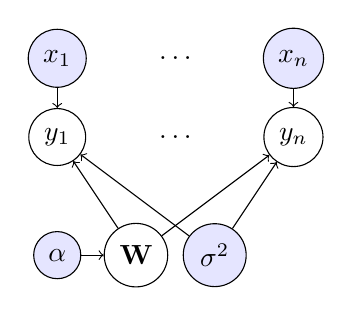
\begin{tikzpicture}
	\draw (0,0) node[shape=circle, 
					 draw=black,
					 fill=blue,
					 fill opacity = 0.1,
					 text opacity = 1.0](x1){$x_1$};
	\draw node[below of = x1, 
			   shape=circle, 
			   draw=black](y1){$y_1$};
	
	\draw (1.5, 0) node[](txt){$\dots$};
	\draw node[below of=txt](txt){$\dots$};
	
	\draw (3,0) node[shape=circle, 
					 draw=black,
					 fill = blue,
					 fill opacity = 0.1,
					 text opacity = 1.0](xn){$x_n$};
	\draw node[below of = xn, 
			   shape=circle, 
			   draw=black](yn){$y_n$};
	
	\draw [->](x1) -- (y1);
	\draw [->](xn) -- (yn);
	
	\draw (0, -2.5) node[shape=circle, 
					 draw=black,
					 fill=blue,
					 fill opacity = 0.1,
					 text opacity = 1.0](alpha){$\alpha$};
	\draw (1, -2.5) node[draw=black, shape=circle](w){$\textbf{W}$};
	\draw (2, -2.5) node[shape=circle, 
					 	draw=black,
					 	fill=blue,
					 	fill opacity = 0.1,
					 	text opacity = 1.0](sigma){$\sigma^2$};
	
	\draw [->](w) -- (y1);
	\draw [->](w) -- (yn);
	\draw [->](sigma) -- (y1);
	\draw [->](sigma) -- (yn);
	\draw [->](alpha) -- (w);
\end{tikzpicture}
\end{minipage}
&
\begin{minipage}[c]{0.4\textwidth}
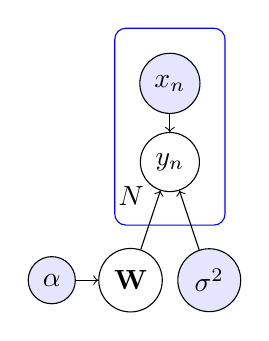
\begin{tikzpicture}
	\draw (1.5,0) node[shape=circle, 
					 draw=black,
					 fill=blue,
					 fill opacity = 0.1,
					 text opacity = 1.0](x1){$x_n$};
	\draw node[below of = x1, 
			   shape=circle, 
			   draw=black](y1){$y_n$};

	\draw [->](x1) -- (y1);
	\draw [draw=blue, rounded corners] (0.8, -1.8) rectangle
		 node[pos = 0.15]{$N$} ++(1.4, 2.5);
		
	\draw (0, -2.5) node[shape=circle, 
					 draw=black,
					 fill=blue,
					 fill opacity = 0.1,
					 text opacity = 1.0](alpha){$\alpha$};
	\draw (1, -2.5) node[draw=black, shape=circle](w){$\textbf{W}$};
	\draw (2, -2.5) node[shape=circle, 
					 	draw=black,
					 	fill=blue,
					 	fill opacity = 0.1,
					 	text opacity = 1.0](sigma){$\sigma^2$};
	
	\draw [->](w) -- (y1);
	\draw [->](sigma) -- (y1);
	\draw [->](alpha) -- (w);
\end{tikzpicture}
\end{minipage}
\end{tabular}
\caption{Bayesian networks for Bayesian polynomial regression.
Left is long, expanded network. Right uses shorthand notation.}
\label{fig:exmpl_BN_poly_regr}
\end{figure}

\noindent
From the network we could then marginalize towards $\textbf{W}$ or
towards $Y_i$:
\begin{equation}
p(\textbf{W} \mid \textbf{Y}) 
= \frac{p(\textbf{W})\prod_{i=1}^{m}p(Y_i \mid \textbf{W})}{p(\textbf{Y})}
\end{equation}
\begin{equation}
p(Y_i \mid \textbf{W}, \textbf{Y}^i) 
= \frac{p(\textbf{W} \mid \alpha)\prod_{i=1}^{m}
	p(Y_i \mid \textbf{W})}{p(\textbf{W}, \textbf{Y}^i)}
\end{equation}

\noindent
This network is not particularly interesting as we already have
the observations $\textbf{y}={y_1, \dots, y_n}$. In order to 
predict a new data point $x_{n+1}$ we can expand our model as follows:
\begin{equation}
p(Y_{n+1}, \textbf{W}, \textbf{Y}\mid x_{n+1})
	= p(\textbf{W})p(Y_{i+1}\mid \textbf{W}, x_{n+1})
	\prod_{i = 1}^{n}p(Y_i\mid \textbf{W})
\end{equation}

\noindent
The Bayesian network corresponding with this model would be an
extension of the model in figure \ref{fig:exmpl_BN_poly_regr}.

\begin{figure}[h!]
\centering

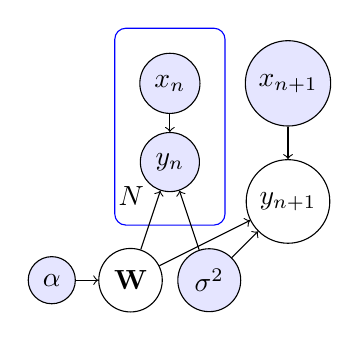
\begin{tikzpicture}
	\draw (1.5,0) node[shape=circle, 
					 draw=black,
					 fill=blue,
					 fill opacity = 0.1,
					 text opacity = 1.0](x1){$x_n$};
	\draw node[below of = x1, 
			   shape=circle, 
			   draw=black,
			   fill = blue,
			   fill opacity = 0.1,
			   text opacity = 1.0](y1){$y_n$};
			   
	\draw (3,0) node[shape=circle, 
					 draw=black,
					 fill=blue,
					 fill opacity = 0.1,
					 text opacity = 1.0](xn1){$x_{n+1}$};
	\draw (3, -1.5)node[shape=circle, 
			   draw=black](yn1){$y_{n+1}$};

	\draw [->](x1) -- (y1);
	\draw [->](xn1) -- (yn1);
	
	\draw [draw=blue, rounded corners] (0.8, -1.8) rectangle
		 node[pos = 0.15]{$N$} ++(1.4, 2.5);
		
	\draw (0, -2.5) node[shape=circle, 
					 draw=black,
					 fill=blue,
					 fill opacity = 0.1,
					 text opacity = 1.0](alpha){$\alpha$};
	\draw (1, -2.5) node[draw=black, shape=circle](w){$\textbf{W}$};
	\draw (2, -2.5) node[shape=circle, 
					 	draw=black,
					 	fill=blue,
					 	fill opacity = 0.1,
					 	text opacity = 1.0](sigma){$\sigma^2$};
	
	\draw [->](w) -- (y1);
	\draw [->](sigma) -- (y1);
	\draw [->](alpha) -- (w);
	\draw [->](sigma) -- (yn1);
	\draw [->](w) -- (yn1);
\end{tikzpicture}
\end{figure}

\noindent
To make this example more clear. We could for example assume several
conditional probability distributions. Take for example 
$p(Y_i \mid \textbf{W})$, in the case of polynomial regression
it could for instance signify:
\begin{equation}
p(Y_i \mid \textbf{W}, x_i) = \mathcal{N}\big(f(\textbf{W}, x_i), V\big)
\end{equation}
The prior over $\textbf{W}$ could be chosen as a Gaussian with
zero mean and some diagonal variance matrix:
\begin{equation}
p(\textbf{W} \mid \alpha) = \mathcal{N}\big( \textbf{0}, \alpha \ID\big)
\end{equation}
\end{exmp}

\section{Discrete variables in Bayesian networks}
We've seen Bayesian networks as defining a joint probability
over a set of random variables $\textbf{X}$. We can apply
the Bayesian network principle to a set of discrete variables.
In fact, Bayesian networks are usually introduced as a way to
compactly define a distribution over discrete variables.
The rest of this chapter, we will consider the random variables
of a Bayesian network as discrete. However, keep in mind that 
this doesn't have to be the case.

\subsection{Full joint probabilities}
When dealing with discrete variables, one usually uses multinomial 
distributions. Given a discrete variable $X$, which can take on
$K$ values from $1$ to $K$ with probabilities 
$\mu = \{\mu_1, \dots, \mu_K\}$. The probability 
distribution of $X$ is given by:
\begin{equation}
p(X \mid \mu) = \prod_{i=1}^{K} {\mu_i}^{x_i}
\end{equation}
Where $x_i$ indicates whether $X$ has taken value $i$. To define
this distribution, one would need exactly $K - 1$ parameters. We
subtract $1$ as the condition $\sum \mu_i = 1$ must hold and we
lose a degree of freedom. For a single variable this is not yet a
problem. However, what happens when we have a join distribution over
$m$ variables, where each variable can assume $K$ values?
In this case the probability distribution would look as follows:
\begin{equation}
p(X_1, \dots, X_m) = p(X_1)p(X_2 \mid X1)\dots p(X_m \mid X_1, \dots, X_{m-1})
\end{equation}
For each $p(X_i \mid X_1, \dots, X_{i-1})$ we need exactly $K^{i-1}(K - 1)$
parameters to define it. We derive it mathematically:
\begin{equation}
\sum_{i=1}^{m} K^{i-1}(K - 1) = K^m -1
\end{equation}
The proof for this equation can be found in the definitions
section at the start.
In total we obtain exactly $K^m - 1$ parameters
needed to fully define the joint distribution. This is of course
unmanageable in any real world context. There are several ways 
one could combat this. One way is by imposing an independence structure
in the form of Bayesian networks. Take for example a joint probability
distribution over $\textbf{X} = \{A, B, C, D\}$, each taking values in
$\{1, 10\}$. This network would consist of $10^{4} - 1 = 9999$ 
parameters. If we use for example the network in figure
\ref{fig:BN_exmaple_params}, we would only use $9 + 90 + 900 + 90 
= 1089$ 
parameters.
\begin{figure}[h!]
\centering
\begin{minipage}[c]{0.3\textwidth}
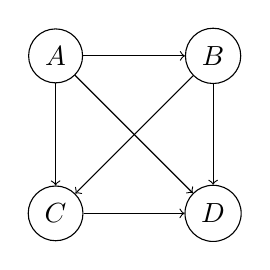
\begin{tikzpicture}
	\draw (0, 0) node[draw = black,
					  shape = circle
			   ](A){$A$};
	\draw (2, 0) node[draw = black,
					  shape = circle
			   ](B){$B$};
	\draw (0, -2) node[draw = black,
					  shape = circle
			   ](C){$C$};
	\draw (2, -2) node[draw = black,
					  shape = circle
			   ](D){$D$};
			   
	\draw[->] (A) -- (B);
	\draw[->] (A) -- (C);
	\draw[->] (A) -- (D);
	
	\draw[->] (B) -- (C);
	\draw[->] (B) -- (D);
	
	\draw[->] (C) -- (D);
\end{tikzpicture}
\end{minipage}
\begin{minipage}[c]{0.3\textwidth}
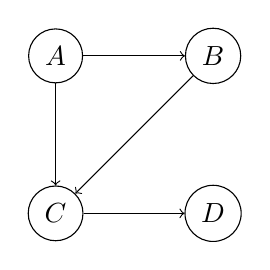
\begin{tikzpicture}
	\draw (0, 0) node[draw = black,
					  shape = circle
			   ](A){$A$};
	\draw (2, 0) node[draw = black,
					  shape = circle
			   ](B){$B$};
	\draw (0, -2) node[draw = black,
					  shape = circle
			   ](C){$C$};
	\draw (2, -2) node[draw = black,
					  shape = circle
			   ](D){$D$};
			   
	\draw[->] (A) -- (B);
	\draw[->] (A) -- (C);
	
	\draw[->] (B) -- (C);
	
	\draw[->] (C) -- (D);
\end{tikzpicture}
\end{minipage}
\caption{Example of fully connected Bayesian network (left) and
not fully connected Bayesian network (right).}
\label{fig:BN_exmaple_params}
\end{figure}

\noindent
Using Bayesian networks, we can
easily reduce the amount of parameters even further. For example
by parameter sharing between connections, referred to as \textit{tying}
parameters. Take for example the connections $p(B \mid A)$ and 
$p(D \mid C)$. If we assume they share parameters we would instead
have $9 + 900 + 90 = 999$ parameters. Lastly another simple method
of reducing the number of parameters is by using parameterized models
for example a logistic regression. As an example, take variable $C$
in figure \ref{fig:BN_exmaple_params}. We could define $C$ as:
\begin{equation}
p(C \mid A, B) = \sigma\Big( w_0 + w_1 A + w_2 B \Big)
\end{equation}

\section{Conditional independence by BNs}
An important property in Bayesian networks is conditional independence:
\begin{defn}
Two variables $A$ and $B$ are conditionally independent given $C$ 
if and only if:
\begin{equation}
p(A \mid B, C) = p(A \mid C)
\end{equation}
Intuitively, if we have information about $C$ then any information
we have about $B$ is irrelevant for the outcome of $A$. Conditional
independence shall be denoted as $A \CI B \mid C$.
\end{defn}

\noindent
The significance of conditional independence will become clear later
when looking at inference in Bayesian networks. We can represent 
$A \CI B \mid C$ in a Bayesian network as depicted in figure
\ref{fig:BN_CI_ABC}. This is because 
$p(A, B \mid C) = p(A \mid C)p(B \mid C)$.

\begin{figure}[h!]
\centering
\begin{minipage}{0.3\textwidth}
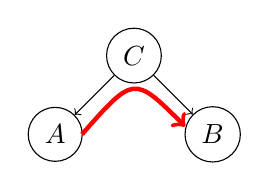
\begin{tikzpicture}
	\draw (0,0) node[draw = black,
					 shape = circle](A) {$A$};
	\draw (1, 1)node[draw = black,
					 shape = circle](C) {$C$};
	\draw (2, 0)node[draw = black,
					 shape = circle](B) {$B$};
					 
	\draw[->] (C) -- (A);
	\draw[->] (C) -- (B);
	
	\draw[red, ->, ultra thick] (0.34,0) .. controls (1, 0.75) .. (1.65,0.1);
\end{tikzpicture}
\end{minipage}
\begin{minipage}{0.3\textwidth}
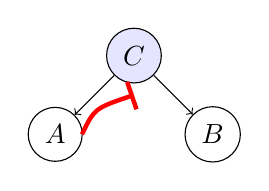
\begin{tikzpicture}
	\draw (0,0) node[draw = black,
					 shape = circle](A) {$A$};
	\draw (1, 1)node[draw = black,
					 shape = circle,
					 fill = blue,
					 fill opacity = 0.1,
					 text opacity = 1.0](C) {$C$};
	\draw (2, 0)node[draw = black,
					 shape = circle](B) {$B$};
					 
	\draw[->] (C) -- (A);
	\draw[->] (C) -- (B);
	
	\draw[red, -|, ultra thick] (0.34,0) .. controls (0.5, 0.33) .. (1,0.5);
	
\end{tikzpicture}
\end{minipage}

\caption{Depiction of $A$ is independent of $B$ given $C$. 
Left, the information can flow from $A$ to $B$, because $C$
is unknown. Right the 
information is blocked, because $C$
is known.}
\label{fig:BN_CI_ABC}
\end{figure}

\noindent
Of course, this conditional independence does not mean $A$ and $B$
are independent variables. If $C$ is not given, information about $A$
may very well influence the outcome of $B$. We notice that information
\textit{travels} from $A$ to $B$ if $C$ is unknown. Conversely, 
information in \textit{blocked} from $A$ to $B$ if $C$ is known.

\section{D-separation}
In this section we have a closer look at the previous observation.
How does information \textit{travel} throughout the Bayesian net
given specific observations? Which variables are conditionally 
independent from each other given a certain set of other variables?
Is there an easy way to verify these by using the DAG?
\\\\
To investigate these questions further, we first look at the 
three building blocks in Bayesian networks. Each of the building
blocks are Bayesian networks with exactly three nodes. For
each of them we will observe how information travels from one
node to another. From there, we can define a notion of conditional
independence between groups of variables in more complex Bayesian
networks.

\subsection{Building block: one}
This 3 node network has already been discussed. Namely the network 
in figure \ref{fig:BN_CI_ABC}. We've already mentioned that $C$
will \textit{block} information flow from $A$ to $B$ if it is given.
We will denote this type of path as $A \leftarrow C \rightarrow B$.
\begin{exmp}
Consider $A=$ whether or not you have a runny nose.
$B = $ Whether or not you have a fever. $C=$ whether or not you 
have the flu. Clearly, if you know you have the flu $C = 1$, then
whether or not you have a runny nose $A = 1$ is independent
from whether or not you have a fever $B = 1$. However, if $C$ is
unknown, one might expect to have a higher chance of a runny nose 
($A = 1$) if you already have a fever ($B = 1$).
\end{exmp}

\noindent
We can verify that, in general $A \not \CI B$:
\begin{equation}\begin{split}
p(A, B) 
	&= \sum_c p(A, B \mid c)p(c)\\
	&= \sum_c p(A \mid c)p(B \mid c)p(c)
\end{split}\end{equation}
This is of course not equal to $p(A)(B)$ in the general case. 
However, with information about $C$ we do find independence:
\begin{equation}\begin{split}
p(A, B \mid c) 
	&= \frac{p(c)p(A \mid c)p(B \mid c)}{p(c)} \\
	&= p(A \mid c) p(B \mid c)
\end{split}\end{equation}
We conclude that $A \not \CI B$ and $A \CI B \mid C$.
\subsection{Building block: two}
The second building block is shown in figure \ref{fig:building_block_two}.
In this case we find a very similar situation as building block one.
If $C$ is known, information is \textit{blocked} from $A$ to $B$.
However, information flows freely from $A$ to $B$ if $C$ is unknown.
We will denote this type as $A \rightarrow C \rightarrow B$.

\begin{figure}[h!]
\centering
\begin{minipage}{0.4\textwidth}
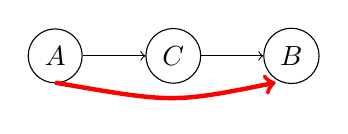
\begin{tikzpicture}

	\draw (0,0) node[draw = black,
					 shape = circle] (A) {$A$};
	
	\draw (3,0) node[draw = black,
					 shape = circle] (B) {$B$};
					 
	\draw (1.5,0) node[draw = black,
					 shape = circle] (C) {$C$};
					 
	\draw[->] (A) -- (C);
	\draw[->] (C) -- (B);
	
	\draw[red, ultra thick, ->] (0, -0.34) .. 
			controls (1.5, -0.6) .. (2.8, -0.34);
\end{tikzpicture}
\end{minipage}
\begin{minipage}{0.4\textwidth}
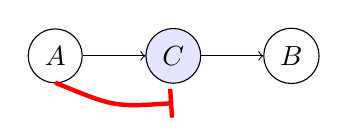
\begin{tikzpicture}

	\draw (0,0) node[draw = black,
					 shape = circle] (A) {$A$};
	
	\draw (3,0) node[draw = black,
					 shape = circle] (B) {$B$};
					 
	\draw (1.5,0) node[draw = black,
					 shape = circle,
					 fill = blue,
					 fill opacity = 0.1,
					 text opacity = 1.0] (C) {$C$};
					 
	\draw[->] (A) -- (C);
	\draw[->] (C) -- (B);
	
	\draw[red, ultra thick, -|] (0, -0.34) .. 
			controls (0.75, -.65) .. (1.5, -0.6);
\end{tikzpicture}
\end{minipage}
\caption{The second building block for D-separation. 
Left, the information can flow from $A$ to $B$, because $C$
is unknown. Right the 
information is blocked, because $C$
is known.}
\label{fig:building_block_two}
\end{figure}
\begin{exmp}
Consider $A=$ whether you are late for the bus. $C =$ whether you are 
late for the train and $B = $ whether you are late for your work. 
Clearly, if you are late for the train ($C = 1$), being late for
for the bus ($A=1$) will not change whether or not you are late
for work ($B = 1$). Conversely, if you were already late for the bus
($A = 1$) you will most likely be late for the train as well ($C=1$).
Eventually causing you to be late for your work ($B =1$). Hence,
information flows from $A$ through $C$ to $B$.
\end{exmp}

\noindent
Mathematically, we verify that in the general case, $A$ and $B$ are
not independent. I.e. $A \not \CI B$:
\begin{equation}\begin{split}
p(A, B) 
	&= \sum_c p(A)p(c \mid A)p(B \mid c) \\
	&= p(A) \sum_c p(c \mid A)p(B \mid c) \\
	&= p(A) p(B \mid A)
\end{split}\end{equation}
In general, $p(B \mid A) \neq p(B)$. In the case $C$ assumes a known
value, $A$ and $B$ are conditionally independent. We verify:
\begin{equation}\begin{split}
p(A, B \mid c) 
	&= \frac{p(A, B, c)}{p(c)}\\
	&= \frac{p(A)p(c \mid A)p(B \mid c)}{p(c)} \\
	&= \frac{p(A)p(c \mid A)}{p(c)} p(B \mid c)\\
	&= p(A \mid c)p(B \mid c)\\
\end{split}\end{equation}
We conclude $A \not \CI B$ but $A \CI B \mid C$.

\subsection{Building block: three}
The final building block for d-separation can be seen in figure
\ref{fig:building_block_three}. In this three node Bayesian network
we observe the opposite. If $C$ is not observed, the information
is blocked by $C$. However, if $C$ is known, information can flow
from $A$ to $B$. This type will be denoted as $A \rightarrow C
\leftarrow B$

\begin{figure}[h!]
\centering
\begin{minipage}{0.4\textwidth}
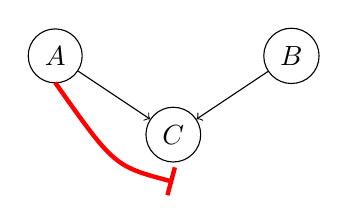
\begin{tikzpicture}

	\draw (0,0) node[draw = black,
					 shape = circle] (A) {$A$};
	
	\draw (3,0) node[draw = black,
					 shape = circle] (B) {$B$};
					 
	\draw (1.5,-1) node[draw = black,
					 shape = circle] (C) {$C$};
					 
	\draw[->] (A) -- (C);
	\draw[->] (B) -- (C);
	
	\draw[red, ultra thick, -|] (0, -0.34) .. controls (0.75, -1.4) 
			..(1.5, -1.6);
\end{tikzpicture}
\end{minipage}
\begin{minipage}{0.4\textwidth}
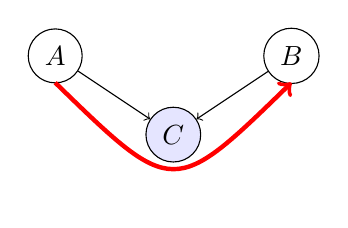
\begin{tikzpicture}

	\draw (0,0) node[draw = black,
					 shape = circle] (A) {$A$};
	
	\draw (3,0) node[draw = black,
					 shape = circle] (B) {$B$};
					 
	\draw (1.5,-1) node[draw = black,
					 shape = circle,
					 fill = blue,
					 fill opacity = 0.1,
					 text opacity = 1.0] (C) {$C$};
					 
	\draw[->] (A) -- (C);
	\draw[->] (B) -- (C);
	
	\draw[red, ultra thick, ->] (0, -0.34) .. controls (1.5, -1.8) 
			..(3, -0.34);
\end{tikzpicture}
\end{minipage}
\caption{The third building block for D-separation. 
Left, the information is blocked from $A$ to $B$, because $C$
is unknown. Right the information can flow from $A$ to $B$, 
because $C$ is known.}
\label{fig:building_block_three}
\end{figure}

\begin{exmp}
Consider $A = $ whether or not your car break fails. $B =$ whether or not
your car motor has failed. Finally, consider $C = $ whether or not
you had a car accident. If you don't know whether or not you have a 
car crash ($C$ unknown), then gaining information about your motor 
($B = 1$) will not change the probability of your breaks failing 
($A = 1$). However, assume now that we know that we know that we had
a car crash ($C = 1$). Clearly if we know it wasn't caused by motor
failure ($B = 0$), then it was most likely caused by break failure 
($A = 1$). Hence, information flows from $B$ to $A$ since we know
$C$.
\end{exmp}

\noindent
Let's verify that information gets blocked if $C$ is unknown:
\begin{equation}\begin{split}
p(A, B) 
	&= \sum_c p(A)p(B)p(c \mid A, B)\\
	&= p(A) p(B) \\
\end{split}\end{equation}
We now show the converse. Given $C$, information can freely flow
from $A$ to $B$:
\begin{equation}\begin{split}
p(A, B \mid c) 
	&= \frac{p(A, B, c)}{p(c)} \\
	&= \frac{p(A)p(B)p(c \mid A, B)}{p(c)}
\end{split}\end{equation}
In general $A \not \CI B \mid C$.

\subsection{D-separation}
So why did we consider these three graphs in the first place?
Usually our Bayesian networks do not consist out of three random
variables. Instead, networks usually consist of thousands of
random variables. D-separation is a useful tool to graphically
verify whether two variable sets $A$ and $B$ are conditionally 
independent given a set of observations $C$.

\begin{defn}[D-separation]
Given a Bayesian network $(G, \Theta)$ over variables $\textbf{X}$.
Two variable sets $A \subset \textbf{X}$ and $B \subset \textbf{X}$ 
are D-separated given observed variable set $C \subset \textbf{X}$ 
iff for each undirected path $P = P_1\dots P_n$ 
from set $A$ to set $B$, the information flow is 
\textit{blocked}. Either by an observed variable $O \in C$ or
by a missing observed variable $O \notin C$. Concretely, for 
each sub-path $P' = P_iP_{i+1}P_{i+2} \in P$:

\begin{itemize}
\item $P'$ is of type $P_i \leftarrow P_{i+1} \rightarrow P_{i+2}$ 
	and $P_{i+1} \in C$ OR
\item $P'$ is of type $P_i \rightarrow P_{i+1}\rightarrow P_{i+2}$ 
	and $P_{i+1} \in C$ OR
\item $P'$ is of type $P_i \rightarrow P_{i+1}\leftarrow P_{i+2}$
	and $(Des(P_{i+1}) \cup \{P_{i+1}\}) \cap C = \emptyset$
\end{itemize}
\end{defn}


\begin{prop}[D-separation implies conditional independence]
Given a Bayesian network $(G, \Theta)$ over random variables
$\textbf{X}$. If variable set $A\subset \textbf{X}$ and 
$B\subset \textbf{X}$ are D-separated given $C \subset \textbf{X}$,
then it holds that $A \CI B \mid C$ in the joint distribution.
\begin{equation}
Dsep(A, B \mid C) \implies A \CI B \mid C
\end{equation}
\end{prop}

\noindent
While a proof would justify this property, intuitively it
makes a lot of sense. By the property of information flow 
in the three building blocks (and symmetry of conditional
independence) we can see how this property makes sense.
As an example, let's look at the Bayesian network in figure
\ref{fig:BN_exmpl_dsep}. On the left we find all paths from
$A$ to $D$ blocked. Thus we can state $Dsep(A, D \mid \{C, B\})$.
However, on the right information can travel through 
$A \rightarrow C \leftarrow B$, $C \leftarrow B \rightarrow D$.
Thus we cannot state $Dsep(A, D \mid C)$.

\begin{figure}[h!]
\centering
\begin{minipage}{0.45\textwidth}
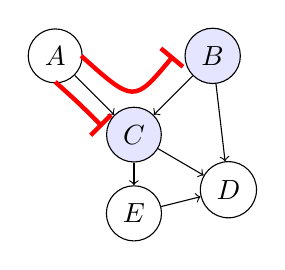
\begin{tikzpicture}
	
	\node [draw, circle] (A) at (0,0){$A$};
	\node [draw, circle,
		   fill = blue,
		   fill opacity = 0.1,
		   text opacity = 1.0] (B) at (2,0){$B$};
	\node [draw, 
		   circle,
		   fill = blue,
		   fill opacity = 0.1,
		   text opacity = 1.0] (C) at (1,-1){$C$};
	\node [draw, circle] (D) at (1,-2){$E$};
	\node [draw, circle] (E) at (2.2,-1.7){$D$};
	
	\draw[->] (A) -- (C);
	\draw[->] (B) -- (C);
	\draw[->] (B) -- (E);
	\draw[->] (C) -- (E);
	\draw[->] (C) -- (D);
	\draw[->] (D) -- (E);
	
	\draw[red, ultra thick, -|] 
		(0, -0.33) .. controls (0.3,-0.6) .. (0.6, -.9);
	\draw[red, ultra thick, -|] 
		(0.33, 0)  .. controls (1,-0.6)   .. (1.5, 0);
	
\end{tikzpicture}
\end{minipage}
\begin{minipage}[c]{0.45\textwidth}
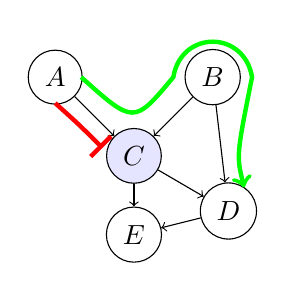
\begin{tikzpicture}
	
	\node [draw, circle] (A) at (0,0){$A$};
	\node [draw, circle] (B) at (2,0){$B$};
	\node [draw, 
		   circle,
		   fill = blue,
		   fill opacity = 0.1,
		   text opacity = 1.0] (C) at (1,-1){$C$};
	\node [draw, circle] (E) at (1,-2){$E$};
	\node [draw, circle] (D) at (2.2,-1.7){$D$};
	
	\draw[->] (A) -- (C);
	\draw[->] (B) -- (C);
	\draw[->] (B) -- (D);
	\draw[->] (C) -- (E);
	\draw[->] (C) -- (D);
	\draw[->] (D) -- (E);
	
	\draw[red, ultra thick, -|] 
		(0, -0.33) .. controls (0.3,-0.6) .. (0.6, -.9);
	\draw[green, ultra thick, ->](0.33, 0)  
		.. controls (1,-0.6) .. (1.5, 0)
		.. controls (1.6, 0.6) and (2.4, 0.6) .. (2.5, 0)
		.. controls (2.3, -1) .. (2.4, -1.4);
	
\end{tikzpicture}
\end{minipage}
\caption{Example of D-separation in a Bayesian network. 
On the left, all paths between $A$ and $D$ are blocked.
On the right, there is a path $ACBD$ thus no independence. }
\label{fig:BN_exmpl_dsep}
\end{figure}

\subsection{Markov blanket}
Often, one is interested in the conditional probability of 
a certain variable $X$ in a Bayesian network $(G, \Theta)$,
given all other variables. As one might expect, we can exploit
the D-separation property to avoid redundant computation and 
reduce complexity. Indeed, if all variables in the network are
given except for $X$ we find a Bayesian network as in figure
\ref{fig:exmpl_markov_blanket}. We observe through D-separation
that information flow is blocked from $X$ to all other nodes 
except the children, parents and parents of children.

\begin{figure}[h!]
\centering
\begin{tikzpicture}

	\node[cloud, 
		  draw, 
		  cloud puffs = 15, 
		  minimum width = 4cm, 
		  aspect = 1.4](cloud) at (1.15,1.2){parents};
	\draw (0,0) node[draw = black,
			   		 shape = circle,
			   		 fill = blue,
			   		 fill opacity = 0.1,
			   		 text opacity = 1.0](p1){$p_1$};
	\draw (1.15,0) node[](1){$\dots$};
	\draw (2.3,0) node[draw = black,
			   		 shape = circle,
			   		 fill = blue,
			   		 fill opacity = 0.1,
			   		 text opacity = 1.0](p2){$p_n$};
	
	\draw (1.15,-1) node[draw = black,
			   		 	shape = circle](X){$X$};
	\draw (0,-2) node[draw = black,
			   		 shape = circle,
			   		 fill = blue,
			   		 fill opacity = 0.1,
			   		 text opacity = 1.0](c1){$c_1$};
	\draw (1.15,-2) node[](1){$\dots$};
	\draw (2.3,-2) node[draw = black,
			   		 shape = circle,
			   		 fill = blue,
			   		 fill opacity = 0.1,
			   		 text opacity = 1.0](c2){$c_n$};
			   		 
	\draw (-1, -1) node[draw = black,
						shape = circle,
			   		 fill = blue,
			   		 fill opacity = 0.1,
			   		 text opacity = 1.0](U1){$u_1$};
	\draw (3.3, -1) node[draw = black,
						shape = circle,
			   		 fill = blue,
			   		 fill opacity = 0.1,
			   		 text opacity = 1.0](U2){$u_n$};
						
	\node[cloud, 
	  draw, 
	  cloud puffs = 15, 
	  minimum width = 4cm, 
	  aspect = 1.4](cloudC) at (1.15,-3.4){children};
			   		 
	\draw[->] (U1) -- (c1);
	\draw[->] (U2) -- (c2);
		
	\draw[->] (-0.4, 0.8) -- (p1);
	\draw[->] (0.4, 0.64) -- (p1);
	
	\draw[->] (1.9, 0.64) -- (p2);
	\draw[->] (2.7, 0.8) -- (p2);
	
	\draw[->] (p1) -- (X);
	\draw[->] (p2) -- (X);
	
	\draw[->] (X) -- (c1);
	\draw[->] (X) -- (c2);
	
	\draw[->] (c1) -- (-0.37, -2.8);
	\draw[->] (c1) -- (0.37, -2.6);
	
	\draw[->] (c2) -- (1.93, -2.6);
	\draw[->] (c2) -- (2.67, -2.8);
			   		 
	\draw[-|, red, ultra thick] (0.8, -1) -- (0.2, -0.5);
	\draw[-|, red, ultra thick] (1.5, -1) -- (2.1, -0.5);
	\draw[-|, red, ultra thick] (0.84, -1.2) 
		.. controls (0, -1.5) .. (-0.5, -1);
	\draw[-|, red, ultra thick] (1.46, -1.2) 
		.. controls (2.3, -1.5) .. (2.8, -1);
		
	\draw[-|, red, ultra thick] (1, -1.333) -- (0.45, -1.95);
	\draw[-|, red, ultra thick] (1.3, -1.333) -- (1.85, -1.95);
	
\end{tikzpicture}
\caption{Example of Markov blanket. The Markov blanket consists
of children, parents and parents of children. Given the Markov
blanket, all information flow is blocked.}
\label{fig:exmpl_markov_blanket}
\end{figure}

\noindent
\begin{defn}[Markov blanket]
The Markov blanket $B_m(X_i)$ of a node $X_i$ in a Bayesian network
$(G, \Theta)$ over random variables $\textbf{X}=\{X_1, \dots, X_k\}$ 
is defined as:
\begin{equation}
B_m(X_i) = \Bigg(\bigcup_{u \in C(X_i)} Pa(u) \Bigg) \cup Pa(X_i) \cup C(X_i)
	\setminus \{X_i\}
\end{equation}
\end{defn}

\noindent
A nice property of the Markov blanket is the following:
\begin{prop}
Given a Bayesian network $(G, \Theta)$ over $\textbf{X}=\{X_1, 
\dots, X_k\}$, then the conditional probability distribution
of $X_i$ given all other variables $\textbf{X}\setminus \{X_i\}$
is equal to the conditional distribution of $X_i$ given the 
Markov blanket.
\begin{equation}
p( X_i \mid X_{j \neq i}) = p(X_i \mid M_b(X_i))
\end{equation}
\end{prop}

\begin{proof}
The proof is straight forward:
\begin{equation}\begin{split}
p(X_i \mid X_{j \neq i}) 
	&= \frac{p(\textbf{X})}{p(X_{j \neq i})}\\
	&= \frac{\prod_{l=1}^{k}p(X_l \mid Pa(X_l))}
		{\int_{X_i} \prod_{l=1}^{k}p(X_l \mid Pa(X_l))dX_i}
\end{split}\end{equation}
In the denominator, we can pull out any terms which do not
contain $X_i$. We define the following sets for ease of notation:
\vspace{-1em}
\begin{multicols}{2}
\begin{equation}\begin{split}
I_b &= C(X_i) \cup \{X_i\}\\
N_b &= V \setminus I_b\\
\end{split}\end{equation}\break
\begin{equation}\begin{split}
S &= \bigcup_{v \in I_b} Pa(v) \\
S' &= \bigcup_{v \in N_b} Pa(v) \\
\end{split}\end{equation}
\end{multicols}

\noindent
We can then re-write the previous equation:
\begin{equation}\begin{split}
p(X_i \mid X_{j \neq i}) 
	&= \frac{\prod_{l=1}^{k}p(X_l \mid Pa(X_l))}
		{\int_{X_i} \prod_{l=1}^{k}p(X_l \mid Pa(X_l))dX_i}\\
	&= \frac{\prod_{u \in N_b}p(u \mid Pa(u))
			 \prod_{v \in I_b}p(v \mid Pa(v))}
			{\prod_{u \in N_b}p(u \mid Pa(u))
			 \int_{X_i} \prod_{v \in I_b}p(v \mid Pa(v))dX_i}\\
	&= \frac{p(N_b \mid S' \setminus N_b)}
			{p(N_b \mid S' \setminus N_b)}
	   \frac{p(I_b \mid S \setminus I_b)}
			{\int_{X_i}p(I_b \mid S\setminus I_b)dX_i}\\
	&= \frac{p(I_b \mid S \setminus I_b)}
			{\int_{X_i}p(I_b \mid S \setminus I_b)dX_i}\\
	&= p(X_i \mid S \setminus I_b \cup I_b \setminus \{X_i\})\\
	&= p(X_i \mid S \cup I_b \setminus \{X_i\})
\end{split}\end{equation}
We are left to prove that $B_m(X_i) = S \setminus \{X_i\}$:
\begin{equation}\begin{split}
S \cup I_b \setminus \{X_i\} 
	&= \Bigg(\bigcup_{v \in C(X_i) \cup \{X_i\}} Pa(v) \Bigg) 
		\cup I_b \setminus \{X_i\}\\
	&= \Bigg(\bigcup_{v \in C(X_i)} Pa(v) \cup Pa(X_i) \Bigg) 
		\cup C(X_i) \cup \{X_i\} \setminus \{X_i\}\\
	&= \Bigg(\bigcup_{u \in C(X_i)} Pa(u) \Bigg) \cup Pa(X_i) \cup C(X_i)
		\setminus \{X_i\}
\end{split}\end{equation}
We conclude that $p(X_i \mid X_{j\neq i}) = p(X_i \mid M_b(X_i))$.
\end{proof}

\section{Constructing Bayesian networks}
Talk about variable ordering, give an example.

\section{Exact inference in Bayesian networks}
We've seen Bayesian networks and argues their usefulness.
In the previous sections on conditional independence, D-separation
and Markov blankets we've mentioned that these properties are very
useful in performing inference. Especially the Markov blanket, which
suffices to compute the conditional probability distribution for 
any variable $X_i$. This reduces computation time considerably.
However, it remains a \# P-complete problem. We are after all,
summing over an exponential number of configurations.
\\\\
Several exact inference techniques exists. One of them makes 
use of dynamic programming and is referred to as variable 
elimination. Here, one makes smart use of previous computations
to avoid redundant computations. Variable elimination is the most
straight forward exact inference algorithm.
\\\\
The second form of exact inference we will discuss in this section
is one based on message passing. As we will see, this algorithm
is efficient and exact for a subset of Bayesian networks.
While the algorithm works for general Bayesian networks, it
is not efficient in the general case. 
This algorithm is referred to as the 
\textit{sum-product} algorithm or \textit{Belief propagation}.
Before we go into sum-product, however, we need to 
first consider factor graphs. Factor graphs are a graphical  
representation of a factorization of a function over multiple 
variables.

\subsection{Variable elimination}
Variable elimination is in a sense just a fancy name for dynamic
programming and caching computation in Bayesian networks. Let's look
at an example of finding the marginal probability of node $E$ in
the Bayesian network in figure \ref{fig:BN_exmpl_dsep}:
\begin{equation}\begin{split}
p(E) 
	&= \sum_{a,b,c,d} P(a, b, c, d, E)\\
	&= \sum_{a,b,c,d} p(a)p(b)p(c \mid a, b)p(d \mid c, b)p(E \mid c, d)\\
\end{split}\end{equation}
If we were to calculate the probability in this fashion, we would
take a sum over $|A||B||C||D| = k^4$ values. Here $|X|$ denotes the
amount of values $X$ can assume, i.e. $|\Omega_X|$. We assume the 
outcome space of each variable to be $k$. Clearly, in larger networks
this would not scale. We can, however, massage the equation a bit 
to win in computation time. We demonstrate as follows:
\begin{equation}\label{eq:var_elim_derv}\begin{split}
p(E) 
	&= \sum_{a,b,c,d} p(a)p(b)p(c \mid a, b)p(d \mid c, b)p(E \mid c, d)\\
	&= \sum_{b,c,d} p(b)p(d \mid c, b)p(E \mid c, d)
			\sum_a p(a)p(c \mid a, b)\\
	&= \sum_{c, d} p(E \mid c, d)\sum_b p(b)p(d \mid c, b)
			\sum_a p(a)p(c \mid a, b)\\
\end{split}\end{equation}
You might be wondering why doing this is useful at all. Let's 
investigate further. The summation over $A$ is a sum over $k$ 
variables. Next we sum over $B$, which is again a summation over
$k$ variables. Finally, we sum over $k^2$ values. In total we
have summed over $2k + k^2$ values. While it might not seem like
much, this is a considerable amount of savings in larger Bayesian 
networks. In order to understand better what's happening exactly,
figure \ref{fig:visual_var_elim} $\sum_a p(a)(c \mid a, b)$ 
assuming that each variable can take values of $0$ and $1$. 
\begin{figure}[h!]
\centering

\definecolor{a1}{rgb}{0.8, 0.9, 1}
\definecolor{a0}{rgb}{0.99, 0.76, 0.9}
\definecolor{mustard}{rgb}{1.0, 0.86, 0.35}
\definecolor{magicmint}{rgb}{0.67, 0.94, 0.82}
\definecolor{cream}{rgb}{1.0, 0.99, 0.82}
\definecolor{amber}{rgb}{1.0, 0.13, 0.32}
\scalebox{0.8}{
\begin{tikzpicture}
	\node[] (A) {
		\begin{tabular}{|c|}
		\hline
		\rowcolor{lightgray} $p(a)$ \\
		\hline
		\begin{tabular}{l|l}
		$a$ & $p_a$ \\
		\hline
		\rowcolor{a0} 0 & $a_0$ \\
		\rowcolor{a1} 1 & $a_1$ \\
		\end{tabular}\\
		\hline
		\end{tabular}
	};
	

	\node[] (pcab) at (0, -3.5) {
		\begin{tabular}{|c|}
		\hline
		\rowcolor{lightgray} $p(c \mid b, a)$ \\
		\hline
		\begin{tabular}{lll|l}
		$b$ & $c$ & $a$ & $p_c$ \\
		\hline
		\rowcolor{a0}  0 & 0 & 0 & $p_1$ \\
		\rowcolor{a1}  0 & 0 & 1 & $p_2$ \\
		\rowcolor{a0}  0 & 1 & 0 & $p_3$ \\
		\rowcolor{a1}  0 & 1 & 1 & $p_4$ \\
		\rowcolor{a0}  1 & 0 & 0 & $p_5$ \\
		\rowcolor{a1}  1 & 0 & 1 & $p_6$ \\
		\rowcolor{a0}  1 & 1 & 0 & $p_7$ \\
		\rowcolor{a1}  1 & 1 & 1 & $p_8$ \\
		\end{tabular}\\
		\hline
		\end{tabular}
	};
	
	\node[] (prod) at (5.2, -1.87) {
		\begin{tabular}{|c|}
		\hline
		\rowcolor{lightgray} $p(c \mid b, a)p(a)$ \\
		\hline
		\begin{tabular}{lll|l}
		$b$ & $c$ & $a$ & $p_cp_a$ \\
		\hline
		\rowcolor{cream}  0 & 0 & 0 & $p_1*a_0$ \\
		\rowcolor{cream}  0 & 0 & 1 & $p_2*a_1$ \\
		\rowcolor{amber}  0 & 1 & 0 & $p_3*a_0$ \\
		\rowcolor{amber}  0 & 1 & 1 & $p_4*a_1$ \\
		\rowcolor{mustard}  1 & 0 & 0 & $p_5*a_0$ \\
		\rowcolor{mustard}  1 & 0 & 1 & $p_6*a_1$ \\
		\rowcolor{magicmint}  1 & 1 & 0 & $p_7*a_0$ \\
		\rowcolor{magicmint}  1 & 1 & 1 & $p_8*a_1$ \\
		\end{tabular}\\
		\hline
		\end{tabular}
	};
	
	\node[] (sm) at (11.2, -1.95) {
		\begin{tabular}{|c|}
		\hline
		\rowcolor{lightgray} $\sum_ap(c \mid b, a)p(a)$ \\
		\hline
		\begin{tabular}{ll|l}
		$b$ & $c$ & $p_cp_a$ \\
		\hline
		\rowcolor{cream}  0 & 0 & $p_1*a_0 + p_2*a_1$ \\
		\rowcolor{amber}  0 & 1 & $p_3*a_0 + p_4*a_1$ \\
		\rowcolor{mustard}  1 & 0 & $p_5*a_0 + p_6*a_1$ \\
		\rowcolor{magicmint}  1 & 1 & $p_7*a_0 + p_8*a_1$ \\
		\end{tabular}\\
		\hline
		\end{tabular}
	};
	
	\node[draw, circle] (times) at (2.5, -2){$\times$};
	\node[draw, circle] (plus) at (8, -2){$\sum$};
	
	\draw[->] (A) -- (times);
	\draw[->] (pcab) -- (times);
	\draw[->] (times) -- (prod);
	\draw[->] (prod) -- (plus);
	\draw[->] (plus) -- (sm);
\end{tikzpicture}
}
\caption{Visualization of $\sum_a p(a)p(c\mid b, a)$.}
\label{fig:visual_var_elim}
\end{figure}

\noindent
In fact, $\sum_a p(a)p(c \mid b, a)$ is very similar as a
local conditional probability. It consists of table, where each
possible configuration of $b$ and $c$ are mapped to a value.
While the local conditional probabilities sum up to $1$,
it does not have to be the case for $\sum_a p(a)p(c \mid b,a)$.
We will denote $\sum_a p(a) p(c\mid b, a)$ as $f_1(b, c)$ and 
continue:
\begin{equation}\begin{split}
p(E) 
	&= \sum_{c, d} p(E \mid c, d)
		\underbrace{\sum_b p(b)p(d \mid c, b)f_1(b, c)}_{f_2(d, c)}\\
	&= \sum_{c, d} p(E \mid c, d)f_2(d, c)\\
	&= f_3(E)
\end{split}\end{equation}

\noindent
By recursively pushing the sum into the product we create 
a computation tree as in figure \ref{fig:comp_tree_var_elim}.

\begin{figure}[h!]
\centering
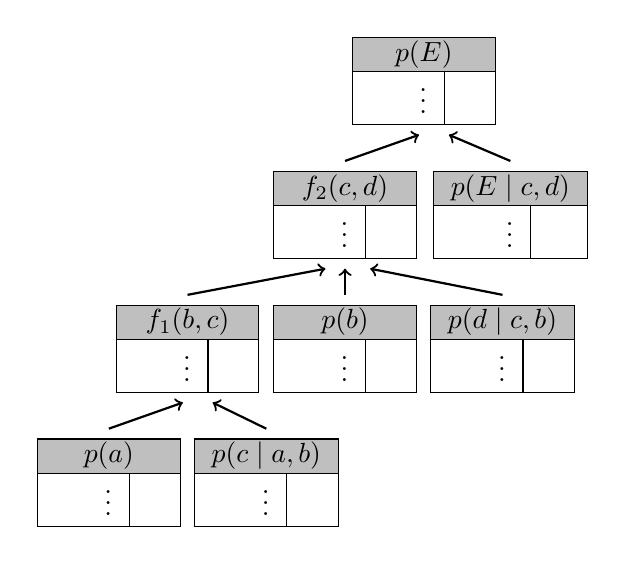
\begin{tikzpicture}

	\node[](pa) at (0,0) {
		\begin{tabular}{|c|}
		\hline
		\rowcolor{lightgray} $p(a)$ \\
		\hline
		\begin{tabular}{ll|l}
		& \vdots & \\
		\end{tabular}\\
		\hline
		\end{tabular}			
	};
	
	\node[](pcab) at (2,0) {
		\begin{tabular}{|c|}
		\hline
		\rowcolor{lightgray} $p(c \mid a, b)$ \\
		\hline
		\begin{tabular}{ll|l}
		& \vdots & \\
		\end{tabular}\\
		\hline
		\end{tabular}			
	};
	
	\node[](f1) at (1,1.7) {
		\begin{tabular}{|c|}
		\hline
		\rowcolor{lightgray}$f_1(b, c)$ \\
		\hline
		\begin{tabular}{ll|l}
		& \vdots & \\
		\end{tabular}\\
		\hline
		\end{tabular}			
	};
	
	\node[](pb) at (3,1.7) {
		\begin{tabular}{|c|}
		\hline
		\rowcolor{lightgray}$p(b)$ \\
		\hline
		\begin{tabular}{ll|l}
		& \vdots & \\
		\end{tabular}\\
		\hline
		\end{tabular}			
	};
	
	\node[](pdcb) at (5,1.7) {
		\begin{tabular}{|c|}
		\hline
		\rowcolor{lightgray}$p(d \mid c, b)$ \\
		\hline
		\begin{tabular}{ll|l}
		& \vdots & \\
		\end{tabular}\\
		\hline
		\end{tabular}			
	};
	
	\node[](f2) at (3,3.4) {
		\begin{tabular}{|c|}
		\hline
		\rowcolor{lightgray}$f_2(c,d)$ \\
		\hline
		\begin{tabular}{ll|l}
		& \vdots & \\
		\end{tabular}\\
		\hline
		\end{tabular}			
	};
	
	\node[](pecd) at (5.1,3.4) {
		\begin{tabular}{|c|}
		\hline
		\rowcolor{lightgray}$p(E \mid c, d)$ \\
		\hline
		\begin{tabular}{ll|l}
		& \vdots & \\
		\end{tabular}\\
		\hline
		\end{tabular}			
	};
	
	\node[](pe) at (4,5.1) {
		\begin{tabular}{|c|}
		\hline
		\rowcolor{lightgray}$p(E)$ \\
		\hline
		\begin{tabular}{ll|l}
		& \vdots & \\
		\end{tabular}\\
		\hline
		\end{tabular}			
	};
	
	\draw[->, thick] (pa.north) -- (f1.265);
	\draw[->, thick] (pcab.north) -- (f1.295);
	
	\draw[->, thick] (f1.north) -- (f2.250);
	\draw[->, thick] (pb.north) -- (f2);
	\draw[->, thick] (pdcb.north) -- (f2.295);
	
	\draw[->, thick] (f2.north) -- (pe.265);
	\draw[->, thick] (pecd.north) -- (pe.295);
\end{tikzpicture}
\caption{The computation tree for variable ordering $a, b, c, d$.}
\label{fig:comp_tree_var_elim}
\end{figure}

\noindent
From equation \ref{eq:var_elim_derv} one might observe that this
is not the only way one could \textit{push} the sum into the product.
In the case of equation \ref{eq:var_elim_derv} the order in which
we pushed the sum into the product is $a$, $b$ then $c$ and $d$.
Note that this variable order might not be optimal to reduce the
computational time. In fact, the computation tree from figure 
\ref{fig:comp_tree_var_elim} might look wildly different depending
on the variable order. A good one might reduce complexity tremendously,
a bad ordering might result in no gain.

\subsection{Factor graphs}
In this section, we introduce factor graphs. Factor graphs are
very similar to Bayesian networks, in the sense that they are
a graphical representation of a factorization of a function. 
In the case of Bayesian networks, we factorize $p(\textbf{X})$
using local conditional probabilities $p(X_i \mid Pa(X_i))$.
In Bayesian networks, each node in the DAG had exactly one
local conditional probability associated with it. 
In factor graphs, however, we have a set $F=\{f_1, \dots, f_k\}$
of factors. Each factor $f_i$ is defined over a subset of the variables
in the original function.

\begin{defn}[Factor graph]
A factor graph over $\textbf{X}= \{X_1, \dots, X_n\}$ for function
$f(\textbf{X})$ is a set of factors $F=\{f_1, \dots, f_k\}$, where
each factor $f_i$ is defined for a subset of $\textbf{X}$. For a factor
graph it holds that:
\begin{equation}
f(\textbf{X}) = \prod_{f_i\in F} f_i(\textbf{X}_i)
\end{equation}
A factor graph is visually represented as a undirected bipartite graph
$G = (V, E)$ consisting of two node types as in figure 
\ref{fig:BN_to_factor} on the right.
The vertices are partitioned into factor nodes $F$ and variable 
nodes $\textbf{X}$, $V = \textbf{X}\cup F$. Factor nodes are 
depicted by a red square and variable nodes depicted by a black
circle containing the variable. Variable nodes only have edges to
factor nodes and vice versa. A factor node is connected to a variable
node if the factor includes this variable:
\begin{equation}
\forall X \in \textbf{X}, \forall f_i \in F: (X, f_i) 
	\in E \Leftrightarrow X \in \textbf{X}_i 
\end{equation}
As factor graphs are undirected, the edge set $E$ is symmetric. 
This means that if there is an edge from $X$ to $f_i$ there is
also an edge from $f_i$ to $X$:
\begin{equation}
\forall v, u \in V: (v, u) \in E \Leftrightarrow (u, v) \in E
\end{equation}
\end{defn}

\noindent
In this definition, $\textbf{X}_i$ denotes the subset of
$\textbf{X}$ over which $f_i$ is defined.
Another similarity with Bayesian networks is the encoding of 
conditional independence. Indeed, conditional independence
in Bayesian networks is encoded by a DAG. By the fact that
the factors $f_i$ are defined over a subset of $\textbf{X}$,
we implicitly leverage structure of our function $f(\textbf{X})$.

\begin{exmp}
Let us consider the joint probability function defined by
the Bayesian network in figure \ref{fig:BN_exmpl_dsep}. Figure
\ref{fig:BN_to_factor} on the left shows this Bayesian network.
We can re-write the Bayesian network over $\textbf{X} = \{
A, B, C, D, E\}$ as a factor graph. Indeed, consider $p(\textbf{X})
= f(\textbf{X})$, we factorize:
\begin{equation}\label{eq:bn_to_factor}\begin{split}
p(A,B,C,D,E) 
	&= p(A)p(B)p(C \mid A, B)p(D \mid C, B)p(E \mid C, D)\\
	&= f_1(A)f_2(B)f_3(A, B, C)f_4(B, C, D)f_5(C, D, E)
\end{split}\end{equation}
How trivial this derivation seems, it shows that any Bayesian
network $(G, \Theta)$ is already by default a factor graph where
$F = \Theta$ for the join distribution $p(\textbf{X})$. However,
not every factor graph is a Bayesian network. Looking at 
\ref{eq:bn_to_factor} we notice that this is not the only way
we could transform the Bayesian network into a factor graph.
Take for example:
\begin{equation}\begin{split}
p(A,B,C,D,E) 
	&= \underbrace{f_1(A)f_2(B)f_3(A, B, C)}_{= f_1(A,B,C)}
			f_4(B, C, D)f_5(C, D, E) \\
	&= f_1(A,B,C)f_4(B, C, D)f_5(C, D, E) \\
\end{split}\end{equation}
This is also a factor graph over $\textbf{X}$ for $p(\textbf{X})$. 
Thus, there are many factor graphs for a given Bayesian network,
depending on which factors are taken together. We draw factor graphs
in a very similar fashion as Bayesian networks. Figure 
\ref{fig:BN_to_factor} shows the Bayesian network transformed into
a factor graph.

\begin{figure}[h!]
\centering
\begin{minipage}{0.4\textwidth}
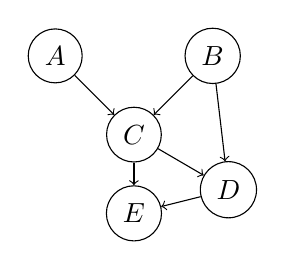
\begin{tikzpicture}
	
	\node [draw, circle] (A) at (0,0){$A$};
	\node [draw, circle] (B) at (2,0){$B$};
	\node [draw, circle,] (C) at (1,-1){$C$};
	\node [draw, circle] (E) at (1,-2){$E$};
	\node [draw, circle] (D) at (2.2,-1.7){$D$};
	
	\draw[->] (A) -- (C);
	\draw[->] (B) -- (C);
	\draw[->] (B) -- (D);
	\draw[->] (C) -- (E);
	\draw[->] (C) -- (D);
	\draw[->] (D) -- (E);
	
	
\end{tikzpicture}
\end{minipage}
\begin{minipage}{0.4\textwidth}
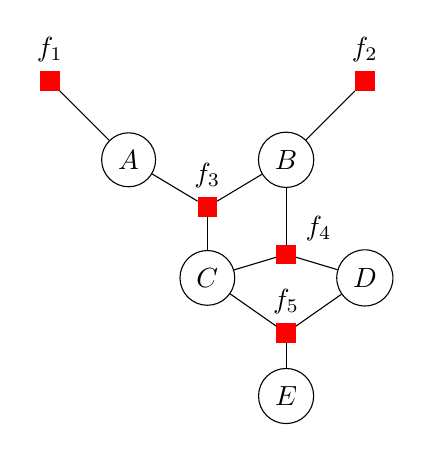
\begin{tikzpicture}
	\node [draw=red, rectangle, 
		   fill=red, label=above:{$f_1$}] (f1) at (-1,1){};
	\node [draw, circle](A) at (0, 0){$A$};
	\node [draw, circle] (B) at (2,0){$B$};
	\node [draw=red, rectangle, 
		   fill=red, label=above:{$f_2$}] (f2) at (3,1){};
		   
	\node [draw, circle,] (C) at (1,-1.5){$C$};
	\node [draw=red, rectangle, 
		   fill=red, label=above:{$f_3$}] (f3) at (1,-0.6){};
		   
	\node [draw, circle] (D) at (3,-1.5){$D$};
	\node [draw, circle] (E) at (2,-3){$E$};
	
	\node [draw=red, rectangle, 
		   fill=red, label=20:{$f_4$}] (f4) at (2,-1.2){};
		   
	\node [draw=red, rectangle, 
		   fill=red, label=above:{$f_5$}] (f5) at (2,-2.2){};
		   
	\draw[-] (f1) -- (A);
	\draw[-] (f2) -- (B);
	
	\draw[-] (f3) -- (A);
	\draw[-] (f3) -- (B);
	\draw[-] (f3) -- (C);
	
	\draw[-] (f4) -- (D);
	\draw[-] (f4) -- (B);
	\draw[-] (f4) -- (C);
	
	\draw[-] (f5) -- (D);
	\draw[-] (f5) -- (E);
	\draw[-] (f5) -- (C);
\end{tikzpicture}
\end{minipage}
\caption{Example of a Bayesian network transformed into a
factor graph.}
\label{fig:BN_to_factor}
\end{figure}

\noindent
The factor graph as seen in figure \ref{fig:BN_to_factor} is a bipartite
graph. The factors do not have edges between other factors. The same holds
for variable nodes. This will play an important role in the sum-product
algorithm.
\end{exmp}

\noindent
We conclude the section on factor graphs by defining what is
meant by the neighbors of a node. In the sum-product algorithm
the neighborhood plays an important role.
\begin{defn}[Neighbors in a factor graph]
Given a factor graph $G = (V, E)$, the neighbors $N(X)$ of a node 
$X \in V$ are defined as all the nodes for which there is a 
connecting edge:
\begin{equation}
N(X) = \{v \in V \mid (v, X) \in E\}
\end{equation}
\end{defn}


\subsection{Sum-product}
We will discuss the sum-product algorithm in context of Bayesian
networks over discrete variables. However, the algorithm does generalize
to continuous variables. 
\\\\
We start our discussion of the sum-product algorithm by applying it
to a subset of factor graphs. The types of factor graphs we will 
consider at first are the tree graphs. These factor graphs do not
contain loops. An example of a tree structured factor graph is depicted
in figure \ref{fig:tree_factor_graph}. Note this tree graph is not
necessarily derived from a Bayesian network. This graph will be 
the running example throughout this section.

\begin{figure}[h!]
\centering

\caption{The running example of a tree structured factor graph. There are
no loops in tree graphs.}
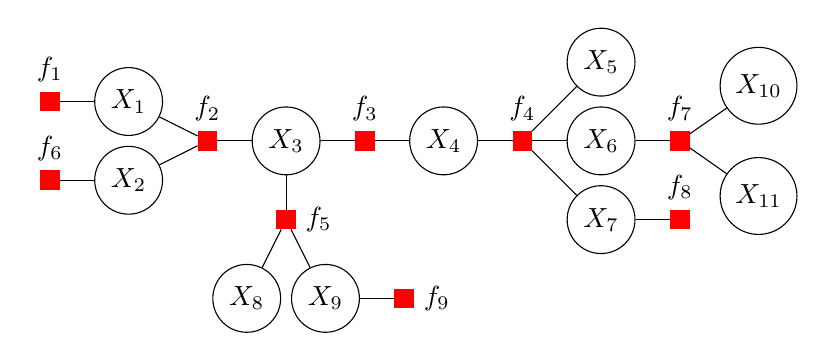
\begin{tikzpicture}
	[
	vn/.style={draw = black, shape = circle},
	fn/.style={draw = red, fill = red, shape = rectangle}
	]
	
	% From left to right
	\node[fn, label=above:{$f_1$}](f1) at (0,0){};
	\node[fn, label=above:{$f_6$}](f6) at (0,-1){};
	\node[vn](X1) at (1,0){$X_1$};
	\node[vn](X2) at (1,-1){$X_2$};
	\node[fn, label=above:{$f_2$}](f2) at (2,-0.5){};
	\node[vn](X3) at (3, -0.5){$X_3$};
	\node[fn, label=above:{$f_3$}](f3) at (4,-0.5){};
	\node[vn](X4) at (5, -0.5){$X_4$};
	\node[fn, label=above:{$f_4$}](f4) at (6,-0.5){};
	\node[vn](X5) at (7, 0.5){$X_5$};
	\node[vn](X6) at (7, -0.5){$X_6$};
	\node[vn](X7) at (7, -1.5){$X_7$};
	\node[fn, label=above:{$f_8$}](f8) at (8, -1.5){};
	\node[fn, label=above:{$f_7$}](f7) at (8, -0.5){};
	\node[vn](X10) at (9, 0.2){$X_{10}$};
	\node[vn](X11) at (9, -1.2){$X_{11}$};
	
	% From up to down
	\node[fn, label=right:{$f_5$}](f5) at (3, -1.5){};
	\node[vn](X8) at (2.5, -2.5){$X_8$};
	\node[vn](X9) at (3.5, -2.5){$X_9$};
	\node[fn, label=right:{$f_9$}](f9) at (4.5, -2.5){};
	
	\draw[-] (f1) -- (X1);
	
	\draw[-] (f2) -- (X1);
	\draw[-] (f2) -- (X2);
	\draw[-] (f2) -- (X3);
	
	\draw[-] (f3) -- (X3);
	\draw[-] (f3) -- (X4);
	
	\draw[-] (f4) -- (X4);
	\draw[-] (f4) -- (X5);
	\draw[-] (f4) -- (X6);
	\draw[-] (f4) -- (X7);
	
	\draw[-] (f5) -- (X3);
	\draw[-] (f5) -- (X8);
	\draw[-] (f5) -- (X9);
	
	\draw[-] (f6) -- (X2);
	
	\draw[-] (f7) -- (X11);
	\draw[-] (f7) -- (X10);
	\draw[-] (f7) -- (X6);
	
	\draw[-] (f8) -- (X7);
	
	\draw[-] (f9) -- (X9);
\end{tikzpicture}
\label{fig:tree_factor_graph}
\end{figure}

\noindent
Let us consider the problem of finding the marginal probability
of a variable $X \in \textbf{X}$, not considering evidence for now.
Mathematically, we want to sum out all the other variables:

\begin{equation}\label{eq:factor_marg}
p(X) = \sum_{\textbf{X}\setminus X}f(\textbf{X})
\end{equation}

\noindent
We can re-write $f(\textbf{X})$ as the product of all the factors
in the factor graph, by definition of factor graphs. However, let
us first partition the factor set $F$. We partition the factors
by considering $X$ as the root node. The partition is then formed
by the factor nodes contained in each sub-tree.
To be more concrete, consider $S(X) = \{G_1, \dots, Gm\}$ the set
of sub trees $G_i = ( V_i \cup F_i, E_i)$ starting at neighbor 
$f_i \in N(X)$. Figure
\ref{fig:factor_subtrees} shows what this means for general factor graphs.
We then partition the set of factors $F$ into the factor sets $F_i$ 
contained in each sub-tree $G_i$. 

\begin{equation}\begin{split}
\bigcup_{G_i \in S(X)} F_i &= F\\
\bigcap_{G_i \in S(X)} F_i &= \emptyset \\
\end{split}\end{equation}
\begin{figure}[h!]
\centering
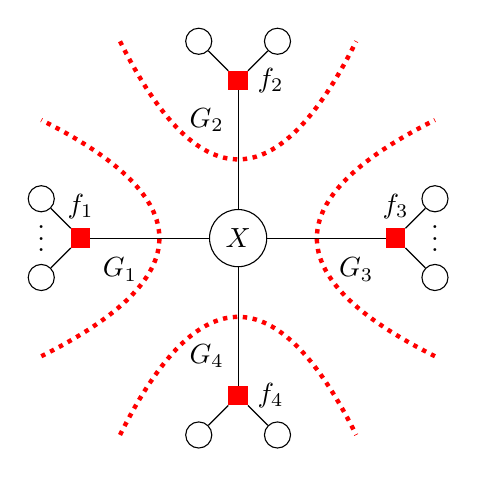
\begin{tikzpicture}
	[
	vn/.style={draw = black, shape = circle},
	fn/.style={draw = red, fill = red, shape = rectangle}
	]
	
	\node[vn](X) at (0,0){$X$};
	
	\node[fn, label=above:{$f_1$}](f1) at (-2, 0){};
	\node[fn, label=right:{$f_2$}](f2) at (0, 2){};
	\node[fn, label=above:{$f_3$}](f3) at (2, 0){};
	\node[fn, label=right:{$f_4$}](f4) at (0, -2){};
	
	\draw[-] (X) -- (f1);
	\draw[-] (X) -- (f2);
	\draw[-] (X) -- (f3);
	\draw[-] (X) -- (f4);
	
	\node[vn] (f11) at (-2.5, 0.5){};
	\node[] (f12) at (-2.5, 0.1){$\vdots$};
	\node[vn] (f13) at (-2.5, -0.5){};
	\draw[-] (f1) -- (f11);
	\draw[-] (f1) -- (f13);
	
	\node[vn] (f21) at (-0.5, 2.5){};
	\node[] (f22) at (0, 2.5){$\hdots$};
	\node[vn] (f23) at (.5, 2.5){};
	\draw[-] (f21) -- (f2);
	\draw[-] (f23) -- (f2);
	
	\node[vn] (f31) at (2.5, 0.5){};
	\node[] (f32) at (2.5, 0.1){$\vdots$};
	\node[vn] (f33) at (2.5, -0.5){};
	\draw[-] (f3) -- (f31);
	\draw[-] (f3) -- (f33);
	
	\node[vn] (f41) at (-0.5, -2.5){};
	\node[] (f42) at (0, -2.5){$\hdots$};
	\node[vn] (f43) at (.5, -2.5){};
	\draw[-] (f41) -- (f4);
	\draw[-] (f43) -- (f4);
	
	\draw[dotted, ultra thick, red, -] (-2.5, -1.5)
		.. controls (-0.5, -0.5) and (-0.5,0.5) 
		.. (-2.5, 1.5);
	\node[](G1) at (-1.5, -0.4){$G_1$};
	
	\draw[dotted, ultra thick, red, -] (-1.5, 2.5)
		.. controls (-0.5, 0.5) and (0.5,0.5) 
		.. (1.5, 2.5);
	\node[](G1) at (-0.4, 1.5){$G_2$};
	
	\draw[dotted, ultra thick, red, -] (2.5, -1.5)
		.. controls (0.5, -0.5) and (0.5,0.5) 
		.. (2.5, 1.5);
	\node[](G1) at (1.5, -0.4){$G_3$};
	
	\draw[dotted, ultra thick, red, -] (-1.5, -2.5)
		.. controls (-0.5, -0.5) and (0.5, -0.5) 
		.. (1.5, -2.5);
	\node[](G1) at (-0.4, -1.5){$G_4$};
\end{tikzpicture}
\caption{Visualization of what is meant by $S(X)$ and $F_i$. Note
that $G_i$ is \textbf{not} a factor graph. This would require 
$X \in F_i \cup V_i$.}
\label{fig:factor_subtrees}
\end{figure}

\begin{exmp}
Take for example $X_3$ as the root for the factor graph in
figure \ref{fig:tree_factor_graph}. We obtain the partitions
$F = \{f_1, f_2, f_6\} \cup \{f_5, f_9\} \cup \{f_3, f_4, f_7, f_8\}$.
\end{exmp}

\noindent
Using the partition of $F$, we re-write $f(\textbf{X})$ from equation
\ref{eq:factor_marg}:

\begin{equation}\begin{split}
f(\textbf{X}) 
	&= \prod_{f_i \in F} f_i(\textbf{X}_i) \\
	&= \prod_{G_i \in S(X)}\prod_{f_i \in F_i} f_i(\textbf{X}_i)\\
	&= \prod_{G_i \in S(X)}F_i(X, V_i)
\end{split}\end{equation}

\noindent
Where $F_i(X, V_i)$ is defined as the product of
all factors in the set $F_i$. Recall that $V_i$ is the set of vertices
of sub graph $G_i$. We now plug in this result into equation
\ref{eq:factor_marg} and push the sum into the product:

\begin{equation}\begin{split}
p(\textbf{X}) 
	&= \sum_{\textbf{X}\setminus X} \prod_{G_i \in S(X)} F_i(X, V_i) \\
	&= \prod_{G_i \in S(X)} \sum_{V_i} F_i(X, V_i) \\
	&= \prod_{G_i \in S(X)} \mu_{f_i \rightarrow X}(X)
\end{split}\end{equation}

\noindent
Where we define $\mu_{f_i \rightarrow X}(X)$ as the sum
$\sum_{V_i} F_i(X, V_i)$, they are referred to as \textit{messages}
from factor $f_i$ to variable $X$. The marginal $p(X)$ is then
defined as the product of all incoming messages as displayed
in figure \ref{fig:messages_to_variable}.
Note, the sum may be pushed into the product
because the sub-graphs $S(X)$ have no overlapping vertices.

\begin{figure}[h!]
\centering
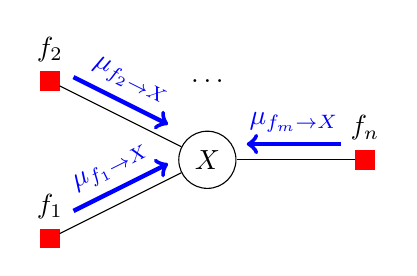
\begin{tikzpicture}
	[
	vn/.style={draw = black, shape = circle},
	fn/.style={draw = red, fill = red, shape = rectangle}
	]
	
	\node[fn, label=above:{$f_2$}](f2) at (0,2){};
	\node[fn, label=above:{$f_1$}](f1) at (0,0){};
	\node[fn, label=above:{$f_n$}](f3) at (4,1){};
	
	\node[vn](X) at (2, 1){$X$};
	
	\node[](dots) at (2, 2){$\dots$};
	
	\draw[-](f1) -- (X);
	\draw[-](f2) -- (X);
	\draw[-](f3) -- (X);
	
	\draw[->,blue, ultra thick, sloped] (0.3, 0.35) -- 
		node[above]{$\mu_{f_1 \rightarrow X}$} (1.5, 0.95);
	\draw[->,blue, ultra thick, sloped] (0.3, 2.05) -- 
		node[above]{$\mu_{f_2 \rightarrow X}$} (1.5, 1.45);
	\draw[->,blue, ultra thick, sloped] (3.7, 1.2) -- 
		node[above]{$\mu_{f_m \rightarrow X}$} (2.5, 1.2);
\end{tikzpicture}
\caption{Messages passed from factor nodes $f_i$ to
a variable node $X$.}
\label{fig:messages_to_variable}
\end{figure}

\noindent



\section{Approximate inference in Bayesian networks}
\subsection{Sampling methods}
